\section{Discussion: Scalability of Connection Numbers}
\label{socksdirect:sec:discussion}

When using commercial RDMA network cards, \sys {} scalability for a large number of connections is limited by the underlying transport layer (i.e., shared memory and RDMA).
To demonstrate that \libipc {} and the monitor are not bottlenecks, this section creates many connections between two processes that reuse RDMA QP and shared memory. An application thread using \libipc {} can create 1.4~M new connections per second, which is 20 times that of Linux and twice that of mTCP \cite {jeong2014mtcp}. The monitor can create 5.3~M connections per second.

Since the number of processes within a host is limited, the number of shared memory connections may not be large.
However, a host may connect to many other hosts, and the scalability of RDMA becomes a problem.
The scalability of RDMA boils down to two issues.
First, RDMA network cards use card memory as a cache to maintain the state of each connection. When there are thousands of concurrent connections, performance is affected by frequent cache misses \cite {mprdma,kaminsky2016design,kalia2018datacenter}.
Because RDMA is traditionally deployed in small and medium-sized clusters, the memory capacity on traditional RDMA network cards is small.
With the large-scale deployment of RDMA in recent years \cite {guo2016rdma}, most network card manufacturers have realized this problem.
Therefore, the memory capacity of recent commercial network cards is getting larger and larger, such as Mellanox ConnectX-5~\cite{connectx-5}, which can store the status of thousands of connections \cite {kalia2018datacenter}. The programmable network card used in this paper even has several terabytes of DRAM~ \cite {mellanox-innova,mellanox-bluefield,smartnic}.
Therefore, this paper predicts that future data centers will not worry too much about the problem of network card cache misses. The next section will propose a scalable transport layer implementation framework based on programmable network cards.
The second issue is that it takes about $30 \mu s$ to establish an RDMA connection in the test platform of this paper, which is important for short connections. This process only involves communication between the local CPU and the network card, so this connection establishment latency can be optimized.

Quality of Service (QoS) under a large number of concurrent connections is also an important requirement for data centers.
Traditional network protocol stacks implement quality of service guarantees in the operating system kernel.
For the hardware transport protocol used in this chapter, offloading data plane performance isolation and congestion control to RDMA network cards is an increasingly popular research direction \cite {peter2016arrakis,zhu2015congestion,lu2017memory,mprdma,mittal2018revisiting}, because data center network cards are becoming more and more programmable  \cite{smartnic,cavium,kaufmann2015flexnic,mellanox-innova,mellanox-bluefield}, and public clouds have already provided QoS in network functions outside of virtual machines \cite {li2016clicknp,panda2016netbricks,floem-osdi18}.

Scalability of connection numbers requires storing the transport layer and packet buffer for each connection. For the transport layer state issue, the next two sections propose two solutions: storing connection states and implementing transport layer processing in programmable network cards or user-level libraries on host CPUs. For the packet buffer issue, the last section proposes multiple socket shared queues, merging the buffers of multiple connections between two processes.

\subsection{Transport Layer Based on Programmable Network Cards}
\label{socksdirect:sec:smartnic}

%\textbf{Communicating with TCP/IP peers.}
%We use a user-space networking stack to communicate with regular TCP/IP peers, but the compatibility may be limited~\cite{yasukata2016stackmap}.
%To solve this problem, after receiving the TCP SYN+ACK, the monitor can create an established kernel TCP connection using TCP connection repair~\cite{tcp-connection-repair}.
%Moreover, if the application and monitor share a network namespace, the monitor can send the kernel file descriptor to the application via Unix domain socket, then \libipc{} can use the file descriptor without delegation to the monitor.

%\textbf{Connecting to many RDMA capable hosts.}
%With a lot of hosts, the network card still suffers from performance degradation due to a large number of connections.
%In contrast, the user-space networking stack alleviates this problem because the network card is stateless.
%We provide a socket option to enable applications to delegate operations to the monitor and use the user-space networking stack even if the peer supports RDMA.
%An application can choose to use RDMA for latency-sensitive and throughput-demanding connections, and the user-space networking stack for others.

This section implements an RDMA network card with scalable number of connections based on the programmable network card, the network packet processing platform in Chapter \ref{chapter:socksdirect}, and the in-memory key-value store in Chapter \ref{chapter:kvdirect}. The main challenge of implementing scalable connections is to access the connection status in the host memory at high throughput when the cache miss rate is high, and to hide the access latency. This is exactly the problem solved in Chapter \ref{chapter:kvdirect}, so this section implements scalable connection status storage based on high-performance key-value storage.

\begin{figure}[htbp]
	\centering
	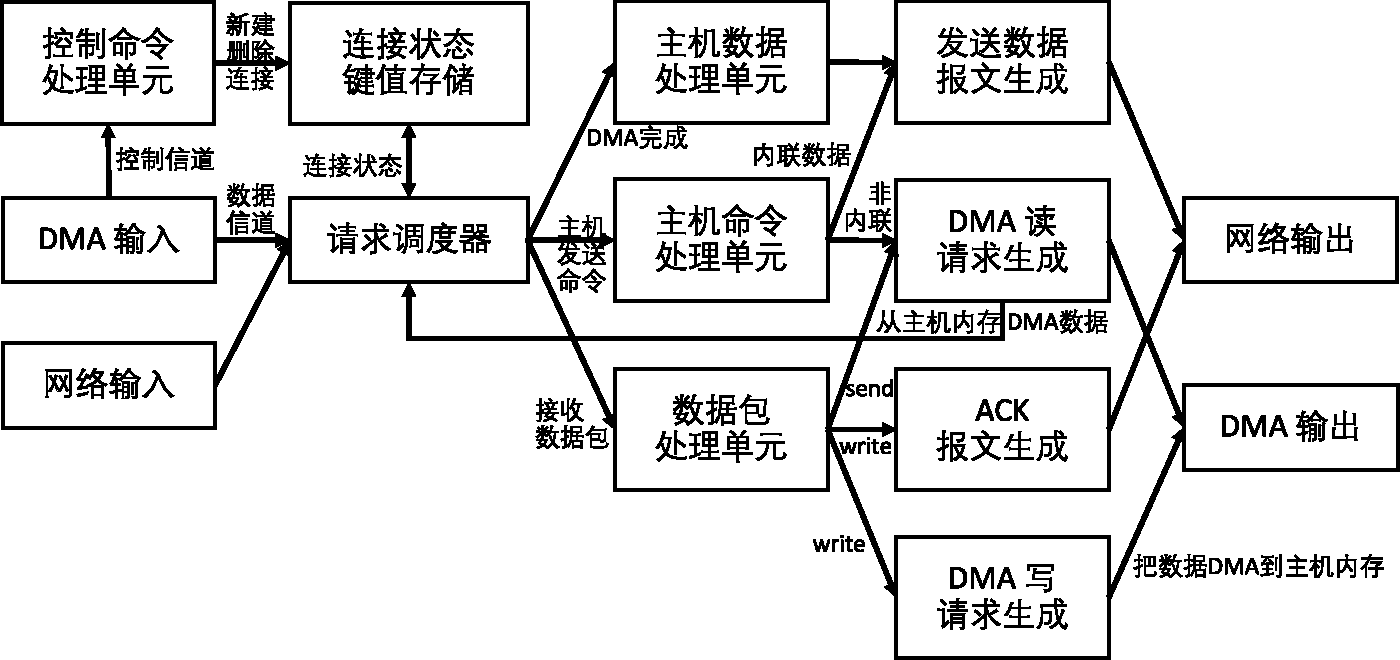
\includegraphics[width=1.0\textwidth]{images/scalable_rdma.pdf}	
	\caption{Scalable RDMA based on programmable network card.}
	\label{socksdirect:fig:scalable-rdma}
\end{figure}

The architecture of the RDMA network card based on the programmable network card is shown in Figure \ref{socksdirect:fig:scalable-rdma}. The RDMA network card needs to handle control and data transmission commands (work requests) from the host, and also needs to handle packets from the network. For control and data transmission commands, the host CPU puts the work request into the work queue in the host memory, and then sends it to the network card through PCIe DMA \cite{kalia2016design}. The packets received through the network interface are also placed in the input buffer of the network card, corresponding to a work request in the work queue. The request scheduler retrieves the connection status information from the connection status key-value store based on the five-tuple information of the packet or the connection number in the host command, and classifies the work request and the current connection status into different work queues inside the network card according to the priority of the connection. Since the processing of RDMA messages is stateful, there may be dependencies between two adjacent packets processed by the same connection. For this reason, the request scheduler records the connections being processed and only schedules work requests for unprocessed connections, which is the same as the way messages with the same key are processed in the key-value store in Chapter \ref{chapter:kvdirect}. For received packets, the receive processing unit processes according to the type of RDMA message. For RDMA one-sided write messages, only need to generate host DMA operations, write data to the corresponding position in the host memory, and reply with an ACK message. For RDMA one-sided read, atomic, and two-sided send messages, it is necessary to read the corresponding data from the host memory before the next operation can be performed. In order to hide the DMA latency of reading from the host memory, after generating the DMA read request for the host memory, a new work request needs to be generated, waiting for the DMA to complete before proceeding to the next step. This new work request is sent back to the request scheduler, and the waiting condition is marked at the same time. When the DMA is completed, the request scheduler will process this new work request, send data to the network or DMA the data to the host memory. The processing of the send command is similar to the processing of the RDMA one-sided read message. The recv command does not require active processing by the network card, but when a two-sided send or one-sided write with immediate message is received from the network, it is necessary to match the corresponding recv work request.

The performance challenge of the above processing flow is that it is difficult to complete the stateful processing of a work request within a single clock cycle, and the work requests of the same connection cannot be processed in parallel, thereby reducing the single-connection throughput. The solution is to pipeline the processing of work requests, each stage handles different parts of the connection status, so there is no data dependency between stages. A data forwarding mechanism is set up within each stage as in Chapter \ref{chapter:kvdirect}, making the state updates that have not been written back to the request scheduler visible to subsequent work requests. In this way, multiple work requests with dependencies from the same connection can be processed concurrently at different stages of the pipeline. For such dependencies that can be resolved through pipelining and data forwarding, the request scheduler does not need to record the dependencies, but considers all such requests as unrelated.

\subsection{CPU-based Transport Layer}
\label{socksdirect:subsec:cpu-transport}

Another solution to implement connection scalability is to implement the transport layer protocol on the host CPU, so that the network card does not need to store the state for each connection, but only needs to implement stateless offloading. A common scheme for network card stateless offloading is to use the send/receive packet interface between the user-mode protocol stack and the network card, rather than the RDMA remote memory access interface. The packet-based implementation can handle a large number of concurrent connections and can be used on virtualization platforms that do not support RDMA. For example, many virtual machine instances in Microsoft Azure cloud do not support RDMA, but support high-performance packet interfaces such as DPDK and LibVMA. The packet-based transport layer can be used on these virtualization platforms.

LibVMA uses a high-performance packet send/receive interface with the network card. The compatibility, performance, and multi-core scalability issues of LibVMA are mainly due to its VFS layer. Therefore, this section uses LibVMA to implement transport layer functions and network card interfaces, replacing the ring buffer and RDMA hardware transport layer in \libipc{}. The structure of the LibVMA \cite{libvma} user-mode socket library is similar to the \libipc{} library in Figure \ref{socksdirect:fig:libsd-architecture}, which is composed of API encapsulation, VFS layer, queue layer, and transport layer. The queue layer and transport layer of LibVMA are composed of the LwIP lightweight TCP/IP protocol stack and the high-speed packet send/receive interface of the Mellnox network card. To use LibVMA, the queue based on the ring buffer in \libipc{} is replaced with the send/receive interface of LwIP. Tests show that the throughput of the LwIP and network card interface parts in LibVMA for sending and receiving small packets is 18M times per second; the throughput of the API encapsulation and VFS layer in \libipc{} is 27M times per second. This means that the throughput of \libipc{} based on LibVMA can reach about 10.8M small packets per second.

To implement zero-copy based on TCP/IP, the LwIP transport layer in LibVMA needs to be modified. For page remapping, the payload of sending and receiving needs to be aligned to the 4~KiB boundary. When sending, \libipc{} assembles a packet composed of two buffers: first is the packet header assembled from the packet header template through the LwIP transport layer, and then the zero-copy payload. \libipc{} uses the scatter-gather support of the network card to let the network card assemble the two buffers into one packet. When receiving, \libipc{} uses a receive work request containing two buffers, first is a 54-byte buffer that can just accommodate the standard TCP/IP packet header, and then the page-aligned payload buffer. As with the design in Section \ref{socksdirect:subsec:lockless-queue}, \libipc{} replenishes the \texttt{recv} work request in time after receiving the packet, keeping the network card always available with the receive buffer.

The above packet interface-based scheme requires the LibVMA library to insert a flow steering rule for each connection, mapping the received packets to the receive work queue. This still requires the network card to maintain the state for each connection, so as shown in the evaluation results in Section \ref{socksdirect:sec:evaluation}, the performance will still decrease when there are many concurrent connections. In order to make the network card completely save the connection state, an unreliable, congestion control-free one-sided RDMA write operation can be implemented with a programmable network card (currently Mellanox RDMA network cards do not support one-sided RDMA based on unreliable datagrams). The one-sided RDMA write operation contains the memory address on the remote host, so the receiving network card only needs to write the payload into the address specified in the packet through PCIe DMA. This way, the ring buffer design in Section \ref{socksdirect:subsec:lockless-queue} can be applied, and the sender synchronizes the changes in the ring buffer to the receiver through the unreliable channel. The packet loss rate of the RDMA-enabled data center network is very low, so packet loss can be detected by timeout. Specifically, the receiver sends an acknowledgment (ACK) packet as soon as it finds data in the ring buffer; if the sender does not receive the acknowledgment packet after a timeout, it retransmits. To implement window-based congestion control, the sender needs to maintain a send window for each ring buffer (i.e., each connection), and adjust the send window when receiving acknowledgment packets and explicit congestion notifications (ECN). The CPU overhead added by transport layer functions such as packet loss recovery and congestion control is limited. This method can solve the scalability problem of the network card connection number.

\subsection{Multiple Sockets Sharing Queue}
\label{socksdirect:subsec:multiplex-conn}

Many applications establish multiple socket connections between two processes. For example, multiple client threads and server threads of a database may establish pairwise connections. HTTP load balancers often establish a connection for each HTTP request with backend web services. Some other transport layer protocols (such as SCTP) and application layer protocols (such as QUIC and many RPC libraries) also provide multi-connection abstraction. In the traditional design, each connection requires independent buffers, so the number of buffers required is relatively large.

To reduce memory usage and improve memory access locality, as shown in Figure \ref{socksdirect:fig:fork-rdwr}, this paper uses a queue to share all connections between a pair of threads. Each data element in the queue is identified by its file descriptor. By using a queue, the memory usage, random memory access, and cache misses of each socket can be reduced.

\begin{figure}[htbp]
	\centering
	\subfloat[Traditional queue structure.]{
		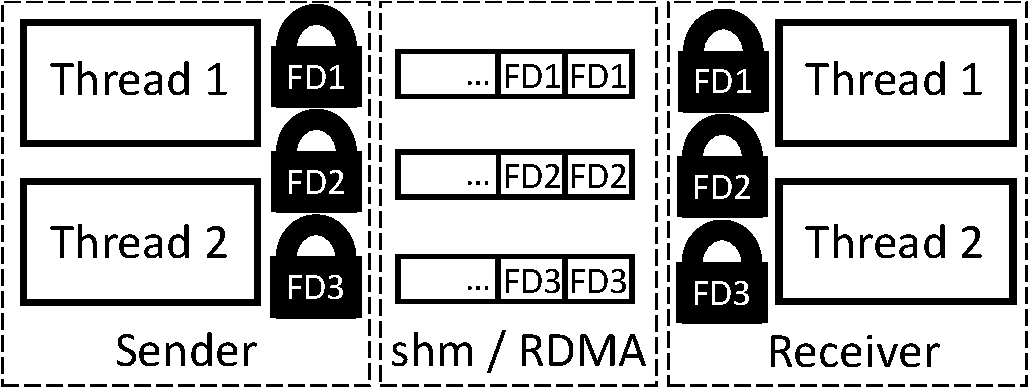
\includegraphics[width=0.6\textwidth]{images/fork_linux}
	}

	\subfloat[Multiple sockets sharing queue structure.]{
		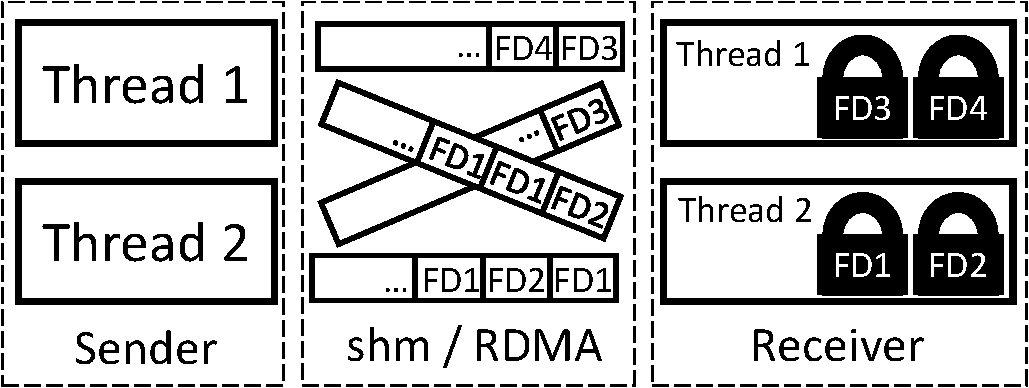
\includegraphics[width=0.6\textwidth]{images/fork_rdwr}
	}
	\caption{Comparison of queue structures. Assume that both the sender and receiver have two threads. First, create peer queues between each pair of sender and receiver threads. Instead of using locks to protect the queue, assign each file descriptor to the receiver thread to ensure ordering. Secondly, data from all connections (file descriptors) is multiplexed through the shared queue, rather than a queue for each file descriptor.}
	\label{socksdirect:fig:fork-rdwr}
\end{figure}

\iffalse
\begin{figure}[htbp]
	\centering
	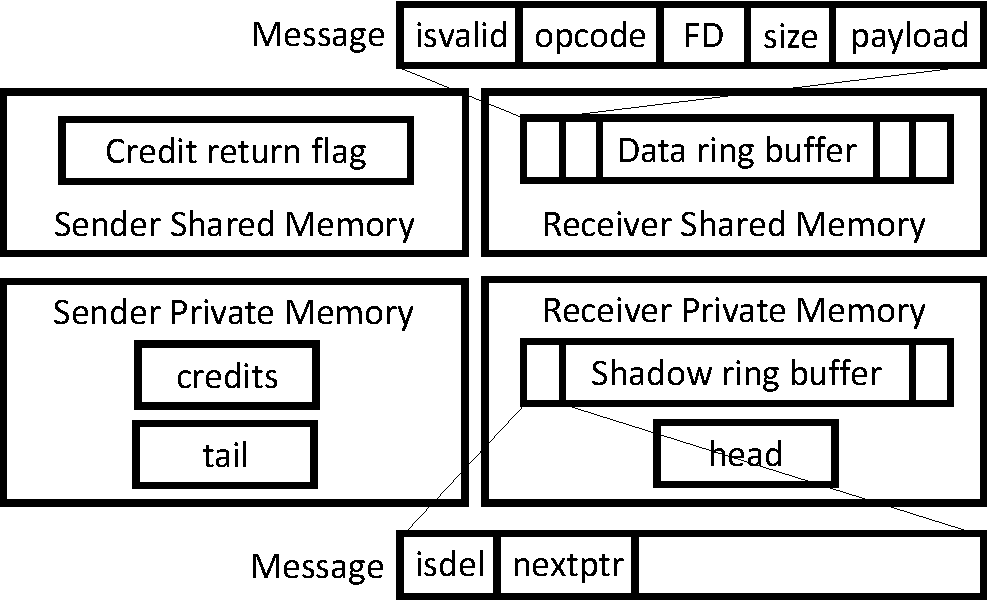
\includegraphics[width=0.8\textwidth]{images/locklessq_new}
	
	\caption{The structure of an inter-process queue.}
	
	\label{socksdirect:fig:locklessq-structure}
\end{figure}
\fi

\textbf{Message format in the queue.}
Based on the traditional queue structure in Section \ref{socksdirect:subsec:lockless-queue}, a file descriptor field is added to the header of each message, indicating the file descriptor of the receiver. In this way, messages from different file descriptors can share a queue. A \textit{next message pointer} field is also added to the header of each message for the following event polling; a \textit{delete} bit is added for the following message retrieval from the middle of the queue.

\textbf{Event polling.}
Maintain a bitmap for each epoll file descriptor set.
When \texttt{epoll\_wait} is called, scan all data queues in turn, and check the file descriptor of each data message in the bitmap.
If the file descriptor is in the bitmap, return an event to the application.
Maintain a global pointer to resume scanning the data queue from the position of the last scan.
To avoid scanning the same message multiple times, set a pointer for each queue to save the position of the last scan.
Since the application may repeatedly perform receive operations on a file descriptor until the queue of the file descriptor is empty, this paper scans and creates a message linked list for each file descriptor to speed up repeated receive operations.
Each file descriptor maintains two pointers, namely the first and last messages scanned but not yet received for this file descriptor.
When a new message of the file descriptor is scanned, the next message pointer field in the message header is updated to point to the newly scanned message, forming a message linked list of the same file descriptor.

\textbf{Retrieving messages from the middle of the queue.}
In order to receive data from any file descriptor, the queue needs to support taking a message from the middle.
Fortunately, this does not happen often. Event-driven applications usually process incoming events in a first-come-first-served order.
For the level-triggered \texttt{epoll\_wait} operation, \libipc{} scans all messages in the queue and returns those messages whose file descriptors have been registered in the epoll file descriptor set.
Therefore, when the application calls \texttt{recv}, the message usually taken is at the head of the queue.

To find a specific file descriptor's message from the middle of the queue, if the message linked list of the file descriptor is not empty, the head of the linked list is the message to be found; if it is empty, it is necessary to traverse the messages in the queue, from the head pointer of the circular buffer to the unallocated space (marked by the \textit{valid} bit). Therefore, when a message is taken from the middle of the queue, its \textit{valid} bit cannot be cleared. Therefore, a \textit{delete} bit is added to each message. When a message is taken from the middle, the \textit{delete} bit is set.

\textbf{Fragmentation consolidation.}
If the application does not receive data from a certain file descriptor for a long time, the free space in the queue will become fragmented.
When there is no available space in the circular buffer, there may still be many deleted messages in it, but because they are located between other messages of file descriptors that have not been received, the space of these messages cannot be used.
When there is no available space in the circular buffer, the sender notifies the receiver to consolidate fragments through the control register in shared memory.
The receiver scans the available space in the circular buffer, concentrates the messages that have not been received, and returns the free space to the sender.

%\textbf{Emergency queue.}
%Control messages may need to be delivered out-of-band when the queue is full. For example, in order to close the receive direction while sending data, the shutdown message should not be blocked by unconsumed data in the queue. To this end, we add an \textit{emergency queue} alongside each data queue.
%A receiver will always retrieve messages in the emergency queue immediately.

The following evaluates the scalability of the number of connections shared by multiple sockets. Before the test, a specified number of connections are pre-established between two processes, and then these connections are used in a round-robin manner to send and receive data in a ping-pong pattern. Figure \ref{socksdirect:fig:eval-connnum-tput} shows the single-core throughput under different concurrent connection numbers. \sys{} can support 100 M concurrent connections with 16 GB of host memory, and the throughput does not decrease at such a high concurrency. In contrast, the performance of RDMA, LibVMA, and Linux decreases rapidly with the increase of the number of connections. For RDMA, the performance drops rapidly after exceeding 512 concurrent connections, which is due to the RDMA transport layer state filling up the network card buffer. Although LibVMA and Linux do not use RDMA as the transport layer, they maintain buffers for each connection, which leads to CPU cache and TLB misses when there are thousands of concurrent connections. In addition, LibVMA installs a connection redirection rule (flow steering rule) for each connection in the network card, which also causes network card cache misses.

\begin{figure}[htbp]
	\centering
	\subfloat[Single-machine throughput.]{                    
		%\begin{minipage}{0.4\textwidth}
		\centering
		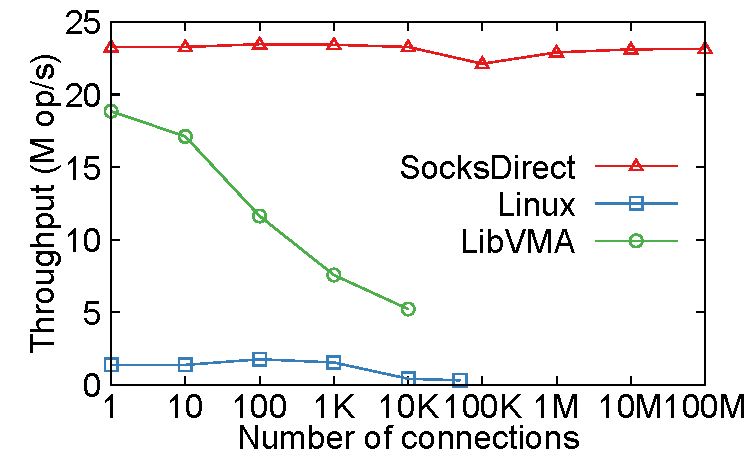
\includegraphics[width=0.5\textwidth]{eval/microbenchmark/connnum-ipc-tput.pdf}
		\label{socksdirect:fig:eval-connnum-ipc-tput}
		%\end{minipage}
	}
	\subfloat[Cross-host throughput.]{
		%\begin{minipage}{0.4\textwidth}
		\centering 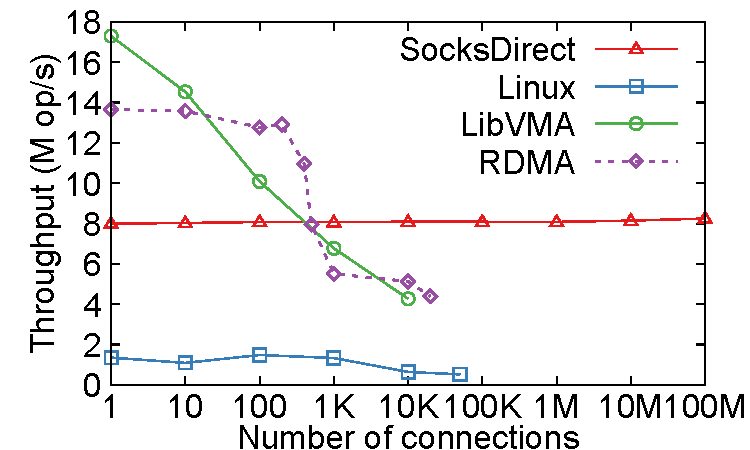
\includegraphics[width=0.5\textwidth]{eval/microbenchmark/connnum-network-tput.pdf}
		\label{socksdirect:fig:eval-connnum-network-tput}
		%\end{minipage}
	}
	
	\caption{Single-core throughput under different concurrent connection numbers.}
	\label{socksdirect:fig:eval-connnum-tput}
\end{figure}


\section{Limitations}
\label{sockdirect:sec:limitation}

In addition to the performance limitations under high concurrency discussed in \S\ref{socksdirect:sec:discussion}, this chapter will discuss the limitations of \sys{} in terms of compatibility and CPU overhead.

\subsection{Compatibility Limitations}



\parab{Transport Layer.}
\sys{} offloads the transport layer mechanism to the RDMA network card. Readers may have some questions about the transport layer mechanism of the RDMA network card. For example, most commercial network cards rely on Priority-based Flow Control (PFC) to eliminate packet loss on Ethernet due to congestion. PFC brings many problems, such as head-of-line blocking, congestion spreading, and even deadlock \cite{guo2016rdma}, making the network difficult to manage and understand. We note that many works aim to improve the performance of the RDMA transport layer. The RDMA congestion control algorithms proposed in recent years \cite{zhu2015congestion,mprdma,mittal2015timely,hpcc} not only improve throughput and latency, but also reduce the number of PFC pause frames. Many advanced packet loss recovery mechanisms \cite{mittal2018revisiting,lu2017memory} also make RDMA no longer need PFC on networks with packet loss. Therefore, we expect future RDMA network cards to provide low-latency and high-throughput transport layers on data center networks with packet loss.

\parab{Priority and Quality of Service Guarantee.}
When multiple threads share the same CPU core, \sys{} uses non-preemptive scheduling. However, to ensure real-time performance and performance isolation, tasks of different priorities in the data center are usually scheduled to be processed on different CPU cores. Processes running on the same CPU core generally handle similar work tasks, and the working processes of existing software (such as Nginx load balancer, Memcached key-value storage, etc.) usually process requests in a first-come-first-served order, without setting process priority.

\parab{Compatibility limitations also exist in other user-space protocol stacks.}
First, like other user-space protocol stacks, \libipc{} uses LD\_PRELOAD to intercept the glibc API of the application program, and cannot intercept direct system calls, so statically linked applications cannot be used.
Second, the sockets created by \sys{} are not visible in the \texttt{/proc} file system, so some network monitoring tools cannot work.
Third, \sys{} lacks some functions of the kernel protocol stack, such as \texttt{netfilter} and traffic control.
However, modern data center network cards already support QoS and ACL offloading ~\cite{mellanox}, so these functions can be offloaded to hardware.

\subsection{CPU Overhead}

\sys{} eliminates many overheads in existing protocol stacks, but introduces some new ones.

\textbf{Monitor polling overhead.}
The polling of the monitor occupies a CPU core. If the monitor is implemented in the kernel and accessed through system calls, the polling overhead will be eliminated, but the overhead of kernel traversal (system calls) and multi-core synchronization in the kernel will increase. Since most control plane operations do not need to go through the monitor, the per-operation overhead added by implementing the monitor in the kernel is acceptable, but it can save the fixed overhead of a CPU core.

\textbf{Idle process polling overhead.}
The cooperative non-preemptive scheduling of \libipc{} has two shortcomings. First, if many processes share a CPU core and the arrival of events is relatively random, the above polling method will wake up a large number of processes without pending events, causing an increase in latency. For this, the kernel's cooperative scheduling needs to become more "intelligent", scheduling processes that have tasks to do based on incoming requests, without reintroducing the series of overheads of the original preemptive scheduling. The core method is to adjust the kernel's scheduling queue based on messages. Consider two situations: first, within a single machine, a dispatch process sends messages to multiple worker processes running on the same CPU core. This is a common communication pattern, such as a task dispatcher distributing tasks to different customer network function processes, or a message source distributing events to multiple subscriber processes. The dispatch process manages the scheduling order of the worker processes. The operating system kernel organizes the worker processes running on the same CPU core into a process group, represented by a bitmap, and maps it to the user space of the dispatch process. After the dispatch process writes data to the shared memory queue, it sets the bit corresponding to the worker process in the bitmap. Modify the kernel scheduler, no longer schedule all ready processes in turn, but scan the bitmap and schedule the next set process. In order to prevent other processes on the same CPU core from starving, the worker process group is treated as a traditional process that is continuously ready and bound to the CPU core. Since non-worker processes are usually in a non-ready (blocked) state, they will not waste CPU time scheduling them.

The second situation is cross-machine communication. At this time, the network card acts as a central dispatcher, and the supported communication mode is arbitrary, not limited to a dispatch process and several worker processes. The event queue of the network card provides the scheduling order of the operating system kernel. The monitor establishes an event queue for each CPU core, which summarizes the completion queue events of all RDMA connections of the processes on the CPU core, written by the network card, and read out by the operating system kernel. The kernel schedules processes according to the order of the event queue, so the scheduled processes are exactly those with events to process. In addition, programmable network cards can observe the length of the event queue on each CPU core, so in a situation where an RDMA message can be distributed to any of the multiple CPU cores, the message can be distributed to the CPU core with the shortest event queue, achieving better load balancing.

\section{Future Work}

\subsection{Interface Abstraction between Applications, Protocol Stacks, and Network Cards}
\label{future:nic-interface}

In this chapter, applications communicate with user-level protocol stacks through socket interfaces, and protocol stacks communicate with network cards through RDMA interfaces. This is to be compatible with existing applications and RDMA network cards. However, applications often have higher-level communication abstractions on the socket layer, such as the key-value storage primitives in Chapter \ref{chapter:kvdirect}, and remote procedure call (RPC), message queue primitives, etc. With the emergence of programmable network cards, the boundary between tasks divided between the host CPU and the network card does not necessarily follow the RDMA interface. Therefore, the interface abstraction between applications, protocol stacks, and network cards can be considered as a whole.

The interface abstraction between applications, protocol stacks, and network cards not only needs to consider performance issues, but also whether it is easy to program. If only considering from the perspective of performance, for existing network cards with smaller memory capacity, a better task division is to implement the transport layer of high-bandwidth and low-latency connections on the network card, and implement the transport layer of a large number of other connections on the host CPU. However, this requires developers to specify which connections need high bandwidth and low latency, which increases the programming burden; or the protocol stack and network card automatically divide and migrate, which will also increase the complexity of the system.

If the protocol stack and applications can not follow the socket interface, there will be a larger design space. Many related works were introduced in Section \ref{socksdirect:sec:background} of this chapter. For example, in terms of zero-copy, if the application can give more hints to the protocol stack, many unnecessary memory copies can be avoided. When the application calls \texttt{send}, it may continue to read and write the send buffer. In order to ensure that the application can read the contents of the buffer, the zero-copy page must be set to read-only, which requires copy-on-write when the receiver in the same host modifies the received content in place. When the application writes to the send buffer, the protocol stack does not know whether the unwritten part of the buffer will be read by the application, so it cannot map an empty page, but needs copy-on-write. This paper intercepts \texttt{memcpy} to optimize the case of whole page writing, but cannot optimize the case where the page is partially written. Many applications actually do not need to read the buffer content after sending. The best solution to the above problems is for the application to inform the protocol stack whether the content of the buffer to be sent needs to be read. This can be achieved by adding an option to the \texttt{send} call, or an additional \texttt{mem\_is\_junk} API.

The message-based RDMA primitives of the network card and the byte-stream-based socket primitives are mismatched. The ring buffer between the sender and the receiver does not need software explicit synchronization in the shared memory of the CPU. But in the shared memory based on one-sided RDMA, software needs to explicitly send RDMA operations to synchronize the two buffers, that is, to synchronize the sender's data to the receiver, and to synchronize the buffer space released by the receiver to the sender. Compared with hardware-implemented coherent shared memory, software explicit synchronization increases CPU overhead. Implementing ring buffer synchronization in hardware can achieve higher throughput, especially when messages are very small.

The current division of transport layer functions between commercial RDMA network cards and host CPUs is not flexible enough. As discussed in Section \ref{socksdirect:subsec:cpu-transport}, the one-sided RDMA operations in Mellanox RDMA network cards only support Reliable Connection (RC) and do not support Unreliable Datagram (UD). This means that if you want to implement the transport layer on the host CPU, you must use two-sided \texttt{send} and \texttt{recv} operations or other packet sending and receiving interfaces provided by the network card, and you cannot use remote memory access primitives. In addition, the functions in the transport layer such as sequential transmission, congestion control, and packet retransmission are also tightly coupled. They either use the hardware implementation fixed by the network card manufacturer, or they are all implemented in software on the CPU. Programmable network cards provide an opportunity to decouple transport layer functions.

If the network card has the ability to handle a large number of concurrent connections, implementing connection establishment in the network card can save the overhead and delay of the CPU in the process of creating connections.

\subsection{Modular Network Protocol Stack}

The network protocol stack is composed of interface abstraction, congestion control, packet loss recovery, Quality of Service (QoS), Access Control List (ACL), packet format, and other components, as shown in Table \ref{socksdirect:tab:network-stack-components}.

\begin{table}[htbp]
	\centering
	\caption{Component selection of the network protocol stack}
	\small
	\begin{tabular}{l|l}
		\hline
		Component & Selection \\
		\hline
		Interface Abstraction & RDMA, BSD socket, StackMap, RPC, Message Queue, \ldots \\
		Congestion Control & TCP, DCTCP, DCQCN, TIMELY, MP-RDMA, IRN, \ldots \\
		Packet Loss Recovery & Go-back-0, Go-back-N, Selective Retransmission, Cut-Payload, \ldots \\
		QoS & Strict Priority, RR, WFQ, Multi-Level Feedback Queue, \ldots \\
		ACL & netfilter, OpenFlow, P4, \ldots \\
		Packet Format & TCP/IP, RDMA, RoCE, RoCEv2, \ldots \\
		\hline
	\end{tabular}
	\label{socksdirect:tab:network-stack-components}
\end{table}

The most representative RDMA protocol stack and TCP protocol stack each implement a set of different components. The RoCEv2 protocol stack, which is widely deployed in data centers, is derived from the RDMA protocol stack, but replaces the packet format to be compatible with the existing data center network's addressing method based on IP addresses and port numbers. \sys{} integrates the components of the two protocol stacks, using the socket interface abstraction of the TCP protocol stack, but the rest of the components all use the corresponding components of RDMA. As discussed in Section \ref{sockdirect:sec:limitation}, the RDMA congestion control and packet loss recovery algorithms used in \sys{} may have fairness issues with standard TCP, and also lack QoS, ACL, and other functions. Therefore, the above components should be modularized and users should be allowed to flexibly combine them. Each component may be implemented in the CPU user mode, CPU kernel mode, or programmable network card. A network protocol stack combination includes the division of tasks between user mode, kernel mode, and programmable network card, as well as the selection of each component. A flexible combination of modular protocol stacks can be implemented using a modular network function programming framework, such as ClickNP in Chapter \ref{chapter:clicknp}.

As shown in Table \ref{socksdirect:tab:api-components}, the interface abstraction of the network protocol stack can be further divided into multiple components. Different combinations of components can form different interface abstractions, suitable for different types of applications, and have different performance characteristics. Many designs of \sys{} aim to implement the interface abstraction of Linux sockets, and pay a performance price for implementing some of these abstractions (for example, to ensure message ordering, the connection needs to be implicitly exclusive to a thread; due to user-managed buffers, non-page-aligned buffers cannot use zero-copy). We look forward to future work proposing a flexible combination of modular network protocol stack interface abstractions.

\begin{table}[htbp]
	\centering
	\caption{Component selection of network protocol stack interface abstraction}
	\small
	\begin{tabular}{l|p{.7\textwidth}}
		\hline
		Component & Selection \\
		\hline
		Addressing Method & IP Address + Port Number, Infiniband Address, Memory Address, Node ID Based on Metadata, \ldots \\
		Connection Abstraction & Byte Stream, Message Stream, Shared Memory, Connectionless, \ldots \\
		Reliability Guarantee & Reliable Order, Tolerate Disorder, Tolerate Packet Loss, Tolerate Errors, \ldots \\
		Connection Sharing Scope & Single Thread, Between Threads, Fork Parent-Child Process, All Processes within Container, \ldots \\
		Connection Sharing Method & Implicit Sharing, Explicit Sharing, Exclusive and Explicit Transfer of Ownership, \ldots \\
		Message Order in Shared Connection & Full Order, Causal Order, No Order, Synchronization Barrier, \ldots \\
		Buffer Management & User Management (RDMA), Protocol Stack Management (socket), User Allocation Protocol Stack Release, Protocol Stack Allocation User Release, \ldots \\
		Notification Method & Blocking, Polling (select), Notify When Ready (epoll), Notify After Completion (aio), Completion Queue (RDMA CQ), \ldots \\
		\hline
	\end{tabular}
	\label{socksdirect:tab:api-components}
\end{table}

%Another promising direction to solve the RDMA concurrency issue is to implement the reliable transport in CPU, and the network card remains stateless. However, RDMA UD does not support one-sided write, so the ring buffer in Sec.~\ref{socksdirect:subsec:lockless-queue} will not work. Existing software RDMA~\cite{soft-roce} has low performance. It would be interesting to co-design software and network card.

%\textbf{Networking stack on other layers.}
%RDMA: lower layer,
%eRPC, message queue, etc: higher layer.

%\section{Related Work}
%\label{socksdirect:sec:related-work}

%Several mostly related works have been discussed in Sec.~\ref{socksdirect:subsec:related-work}.

\iffalse
\parab{Linux kernel optimization.}
One line of research optimizes the kernel stack for higher socket performance. FastSocket~\cite{lin2016scalable} and Affinity-Accept~\cite{pesterev2012improving} scale connection creation to multiple cores, but synchronization is still needed when multiple threads share a socket.
FlexSC~\cite{soares2010flexsc} proposes exception-less system calls to reduce kernel crossing overhead.
Zero-copy socket~\cite{thadani1995efficient,chu1996zero} still needs copy-on-write on senders.
In addition, they fail to remove cache miss and transport overheads.


\parab{New OS stacks.}
Another line of research proposes new OS stacks with modified socket interface, mostly aiming at zero copy and fast event notification. Existing socket applications need modifications to use the new interfaces.
For intra-server connections, Arrakis~\cite{peter2016arrakis} and IX~\cite{belay2017ix} use the network card to forward packets from one process to another. The hairpin latency from CPU to network card is at least two PCIe delays, which is one order of magnitude higher than inter-core cache migration delay. In addition, the data plane switching throughput of a network card is constrained by PCIe bandwidth (Figure~\ref{socksdirect:fig:eval-corenum-tput}).

For inter-server connections, most OS stacks implement transport in software. IX~\cite{belay2017ix} and Stackmap~\cite{yasukata2016stackmap} run in the kernel to enforce QoS policy or preserve protocol compatibility with Linux, while Arrakis~\cite{peter2016arrakis} and SandStorm~\cite{marinos2014network} run in user mode to maximize performance.
RDMA and transport virtualization~\cite{tsai2017lite,niu2017network} also enforce QoS in the hypervisor.
Due to the additional level of indirection, kernel stacks cannot remove kernel crossing, while batched syscalls add latency.
Further, large-scale deployment of kernel-based stacks is more complicated than user-space libraries~\cite{andromeda}.
\sys offloads transport and QoS to network card hardware.
RDMA transport has been deployed in many data centers~\cite{guo2016rdma}, and an emerging line of work~\cite{zhu2015congestion,lu2017memory,mprdma} improves congestion control and QoS in large-scale RDMA deployments.
For flexibility, programmable network cards are being adopted in data centers~\cite{smartnic,cavium}, as they are more efficient than general-purpose CPUs for network processing~\cite{kaufmann2015flexnic,li2016clicknp}.

\parab{User-space socket.}
A third line of research runs socket in user space.
mTCP~\cite{jeong2014mtcp}, Seastar~\cite{seastar}, 
F-stack~\cite{fstack} and LOS~\cite{huang2017high} use a high performance packet I/O framework (\textit{e.g.} netmap~\cite{rizzo2012netmap}, DPDK~\cite{dpdk} and PF\_RING~\cite{pf-ring}) and achieves compatibility with most Linux socket functions and scalability with number of cores and sockets.
LibVMA~\cite{libvma}, OpenOnload~\cite{openonload} and DBL~\cite{dbl} are fully compatible with existing applications. However, they use vendor-specific network card features and do not scale to multiple threads or connections.
In addition, user-space sockets do not support zero copy or efficient multitasking.

Most user-space sockets focus on inter-server and do not optimize for intra-server connections.
FreeFlow~\cite{freeflow} uses shared memory for intra-server communication and RDMA for inter-server, but it provides an RDMA interface.
Existing socket to RDMA translation approaches, \textit{e.g.} SDP~\cite{socketsdirect} and rsockets~\cite{rsockets} are not fully compatible with Linux and do not address scalability challenges.

\fi